%==============================================================================
\section{Background and Problem Definition}
\label{sec:background}
%==============================================================================

This section introduces the background necessary in developing
an oblivious property graph database (GDB).

%------------------------------------------------------------------------------
\subsection{Property Graph Model}
\label{sec:background:graph}
%------------------------------------------------------------------------------

\noindent\textit{\textbf{Data Model.}} A \emph{property graph} $G = (V, E)$ consists of a set of nodes $V$ and a set of directed 
edges $E \subseteq V \times V$. We adopt the property graph model~\cite{robinson2015graph}, 
which represents data using nodes, edge relationships, and associated properties.

\begin{itemize}[leftmargin=*]
\item {Node:} Nodes represent entities in the graph and are grouped by \textit{labels}, 
which denote node types. Within each label, individual nodes are uniquely identified by an id.

\item {Edge relationship:} Edge relationships (referred to simply as \textit{edges} 
hereafter) capture connections between nodes, which may belong to the same or different labels. 
Each edge type is identified by an \textit{edge label}. An edge connects a source node to a 
destination node, and edges are directed. In our model, we restrict any pair of nodes to be 
connected by at most one edge of a given label.

\item {Property:} Nodes and edges can each be associated with a set of properties that store additional descriptive attributes.
\end{itemize}


\noindent\textit{\textbf{Storage Model.}} 
Existing storage models used in oblivious databases introduce challenges when applied to graph 
data. Most oblivious database systems store data either in a key-value format 
~\cite{dauterman2021snoopy, mishra2018oblix} or in a row-oriented tabular 
format~\cite{zheng2017opaque,eskandarian2019oblidb,mavrogiannakis2025obliviator}. For example, 
GraphOS~\cite{chamani2023graphos} represents graph data as key-value pairs organized in an 
oblivious AVL tree. This design incurs an $O(\mathrm{polylog},N)$ overhead for accessing 
\textit{each node or edge}, which becomes a significant performance bottleneck when operating 
on graphs containing millions of nodes and edges.

Although graph data can also be represented using row-wise tables, such a representation is not 
well suited for graph analytics workloads. To better support analytical operations, 
\system uses a disk-based columnar storage layout in which each node or edge property is 
stored in a separate column file. Properties of each node or edge label that are commonly 
queried together are stored together for efficient access.

Unlike plaintext \gdbs, oblivious \gdbs require careful consideration in how to store the
edge lists. Simply storing node-edge relationship in an adjacency list reveals the degree of 
each node even if node and edge ids are encrypted. Hiding node degrees would require padding 
each entry to a worst-case size of $m \times n$, where $m$ denotes the number of edges and $n$ 
the number of nodes, since in the worst case all $m$ edges may originate from a single node.
To avoid this leakage, we instead store adjacency information in a single array-like structure 
sorted by source node ids, thus only revealing the total number of edges $m$ (for a given edge 
label), which we treat as non-sensitive.

Furthermore, following common design practices in plaintext \gdbs such 
as~\cite{janusgraph,feng2023kuzu,deutsch2019tigergraph,sun2015sqlgraph}, we also maintain 
\textit{reverse edges}, stored in sorted order of destination node ids. This reverse index has 
size $m$ and enables efficient bidirectional traversal and parallel processing of graph 
queries. 


\noindent\textbf{\textit{Query Model.}} \system supports Cypher-like queries \cite{francis2018cypher, opencypher} wherein each query specifies the nodes and edges to match 
in the graph with predicates filtering on properties. We categorize graph queries in
two ways:

\begin{itemize}[leftmargin=*]
    \item A \textbf{one-hop query} matches two nodes connected by an edge: (source node) $\rightarrow$ [edge] $\rightarrow$ (destination node). For example, ``find all transactions from accounts with balance $>$ 10000'':
    \begin{center}
    \texttt{(a:Account)-[t:Transaction]$\rightarrow$(b:Account)}\\
    \texttt{WHERE a.balance > 10000}
    \end{center}

    \item A \textbf{$k$-hop query} chains $k+1$ nodes traversing $k$ edges. For example, a 3-hop query might find ``accounts reachable within 3 transactions from a flagged account'':
    \begin{center}
    \small\texttt{(a1:Account)-[t1:Transaction]$\rightarrow$(a2:Account)-[t2:Transaction]\\
    $\rightarrow$}\small\texttt{(a3:Account)-[t3:Transaction]$\rightarrow$(a4:Account)}
    \end{center}
\end{itemize}

The output contains nodes and edges satisfying the query pattern as well as all the predicates. 
In relational terms, a $k$-hop query corresponds to a $(2k+1)$-way join: $k+1$ node tables and $k$ edge tables, joined on foreign key relationships. 

%------------------------------------------------------------------------------
\subsection{System and Threat Model}
\label{sec:background:threat}
%------------------------------------------------------------------------------
We consider a system model where an organization outsources its storage and computational needs to a 
cloud. The organization uploads encrypted graph data to the cloud and issues queries to \system hosted
within a Trusted Execution Environment (TEE) such as Intel TDX~\cite{intel_tdx}, AMD SEV-SNP~\cite{sev2020strengthening}. The TEE provides hardware-enforced isolation: code and data 
inside the TEE are protected from the host operating system, hypervisor, and other software
using an encryption engine with processor-embedded root key as the encryption key. 
TEEs allow application to verify the integrity of software running within the TEE using remote 
attestation.


\system adopts a commonly used model in enclave-based approaches
~\cite{dauterman2021snoopy, krastnikov2020efficient, mishra2018oblix, chamani2023graphos, mavrogiannakis2025obliviator}, where an semi-honest attacker can observe the 
server's encrypted network traffic, manage the software stack outside the enclave, and monitor 
memory accesses both inside and outside the enclave at cache line granularity. However, the 
adversary cannot breach the secure processor or access its secret key. 
The attacker  may leverage observable information to launch side-channel attacks, including 
cache attacks~\cite{brasser2017software, hahnel2017high, moghimi2017cachezoom, 
schwarz2017malware}, branch prediction and paging-based attacks~\cite{lee2017inferring, 
van2017telling, xu2015controlled},  and memory bus snooping~\cite{lee2020off}. Attacks based on 
power consumption and timing analysis are considered out of scope for this model.
The threat model considered in \system differs from the trusted proxy-based oblivious systems
\cite{ahmed2025oasisdb,demertzis2020seal,li2014fast,chang2022towards,chang2021efficient},
which are often termed \textit{single} oblivious systems because the adversary has no access
to the proxy machine that runs the obliviousness scheme, and hence, the scheme's memory
footprint or program control flow is hidden from the adversary. These schemes ensure 
obliviousness of the data accessed from the storage. TEE-based oblivious schemes
are considered \textit{doubly} oblivious because they obfuscate the scheme's memory
or control flow along with obfuscating the data accessed from the storage.

\subsection{Security Definition}
\label{sub:sec-definition}

At a high level, an algorithm is said to be \emph{oblivious} if its externally observable 
behavior does not depend on its input data, beyond explicitly permitted leakage. In particular, 
for any two inputs that are consistent with the same public parameters and produce outputs of 
the same size, an adversary observing the execution should be unable to distinguish which input 
was used. For \system, this requirement translates to ensuring that observable side channels—
such as logical data accesses (e.g., which node entries are selected), physical memory access 
patterns (e.g., which memory locations are touched), and control flow decisions—are independent 
of both the underlying data and the query being executed.

To formalize this notion, we adopt a simulation-based definition. Let $\mathcal{L}$ denote the
allowed leakage of the system. In our setting, $\mathcal{L}$ includes the schema, base table 
sizes of the node and edge labels used in a query, the query structure, and the final result size. We require that any information 
revealed during execution can be simulated using only these public parameters.

We define a security game in which an execution is generated either by the real algorithm 
$\mathsf{Alg}$ or by a polynomial time simulator $\mathsf{Sim}$ that is given only the leakage 
$\mathcal{L}$. An adversary $\mathcal{A}$ observes the resulting execution trace and attempts 
to distinguish between the two cases. The algorithm is considered oblivious if no probabilistic 
polynomial-time (PPT) adversary can succeed in this task with more than negligible advantage.

\begin{definition}
An algorithm $\mathsf{Alg}$ is said to be oblivious with respect to leakage $\mathcal{L}$ if there exists a PPT simulator $\mathsf{Sim}$ such that for all PPT adversaries $\mathcal{A}$,
\[
\left| 
\Pr\left[\mathcal{A}(\mathsf{Trace}_{\mathsf{Alg}}) = 1\right] 
- 
\Pr\left[\mathcal{A}(\mathsf{Trace}_{\mathsf{Sim}(\mathcal{L})}) = 1\right] 
\right| \leq \mathrm{negl}(\lambda),
\]
where $\lambda$ is the security parameter.
\label{sec-def}
\end{definition}

\subsection{Oblivious Primitives}
\label{sub:obl-primitives}

\system leverages a number of oblivious primitives as building blocks, which we describe next.

\noindent\textbf{Oblivious compare and set (\textsc{OCmpSet}):}  
A key requirement for oblivious execution is to eliminate secret-dependent branching,
since conditional control flow may leak information through execution traces.  
Instead, we express conditionals using data-independent bitwise operations that can be
efficiently realized using SIMD instructions.  
Given a secret predicate \texttt{flag}, \textsc{OCmpSet}(\texttt{flag}, $x$, $y$) selects $x$ if \texttt{flag}
is true and otherwise $y$, without revealing the value of \texttt{flag} and whether $x$ or $y$ was selected.

\noindent\textbf{Oblivious sorting (\textsc{OSort}):}  
Oblivious sorting rearranges an input array into sorted order while ensuring that the
sequence of comparisons and memory accesses is independent of the input values.
\system adopts bitonic sorting \cite{batcher1968sorting} due to its deterministic structure and 
strong parallelization properties. Bitonic sort executes a fixed sequence of compare-exchange
operations, yielding a time complexity of $O(n \log^2 n)$ for input size $n$, and
$O((n \log^2 n)/p)$ when parallelized across $p$ threads.  
While asymptotically optimal $O(n \log n)$ oblivious sorting algorithms exist ~\cite{ajtai1983sorting, 
goodrich2014zigzag, gu2025flexway}, they often incur higher constants or exhibit limited scalability when
parallelized~\cite{ngai2024distributed}.  

\noindent\textbf{Oblivious compaction (\textsc{OCompact}):}  
Oblivious compaction takes an array of $n$ elements, each annotated with a binary
predicate (e.g., marked or unmarked), and produces a permutation in which all marked
elements are grouped together while preventing any leakage through memory traces.  
Although linear-time compaction algorithms exist \cite{dittmer2020oblivious,goodrich2011oblivious},
they are often difficult to parallelize and incur high constant overheads. Instead, we use 
ORCompact~\cite{sasy2022fast}, which achieves $O(n \log n)$ complexity while enabling parallel execution.  
ORCompact additionally preserves the relative order of marked elements.



%------------------------------------------------------------------------------
\subsection{Oblivious Multi-Way Joins}
\label{sec:background:joins}
%------------------------------------------------------------------------------

\begin{figure}
    \centering
    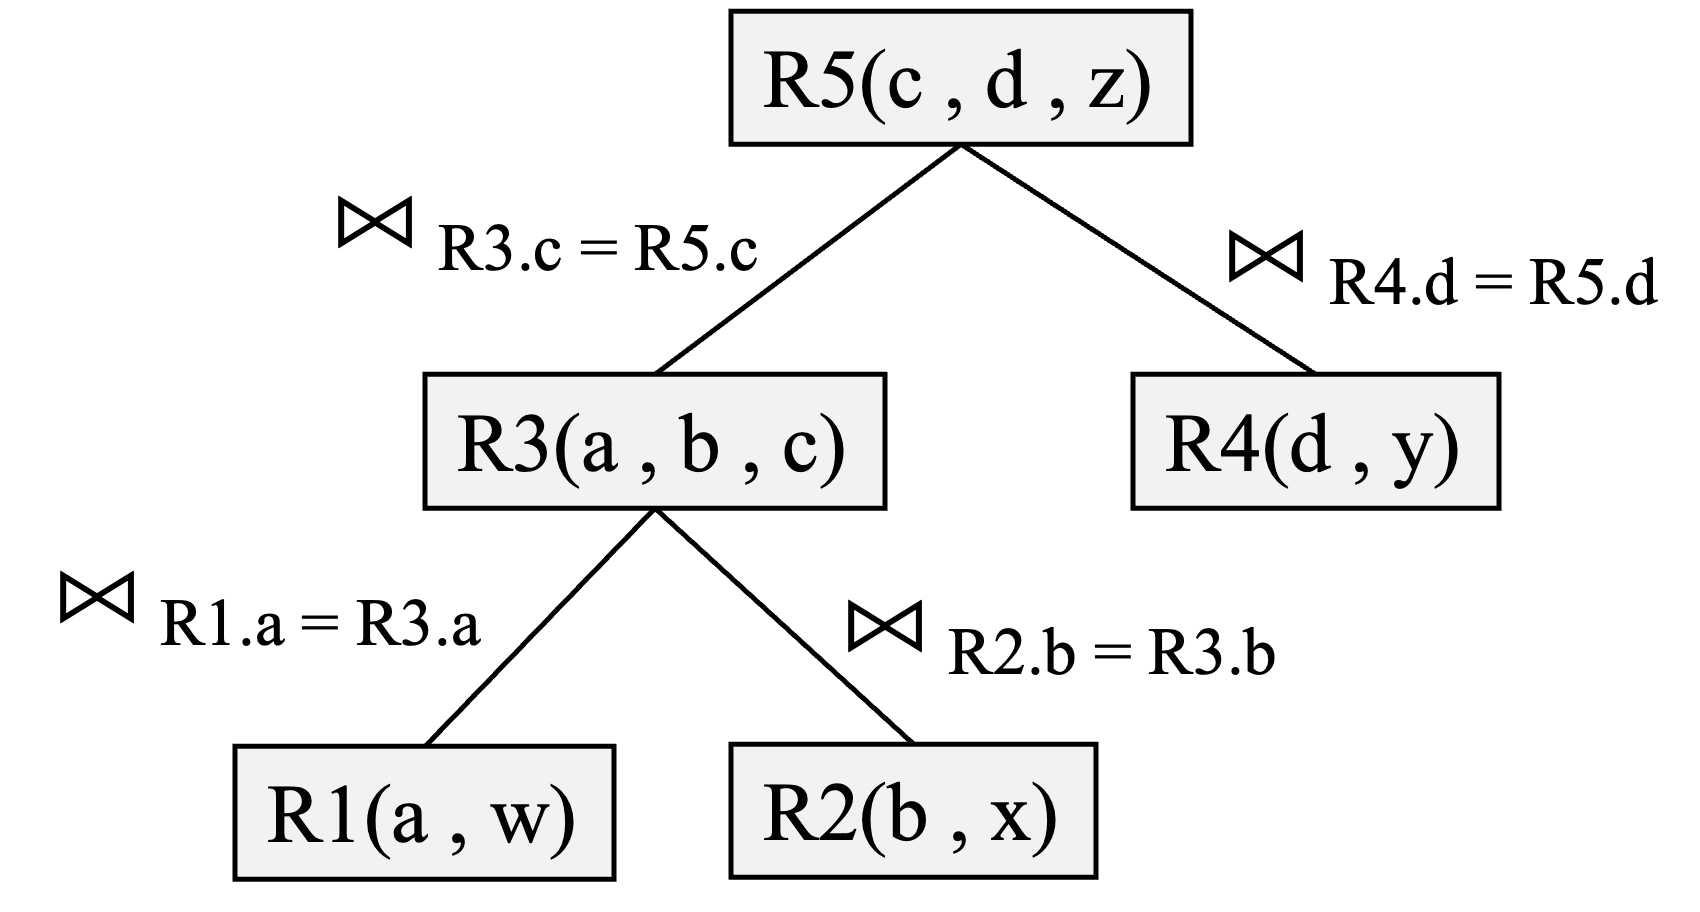
\includegraphics[width=0.5\linewidth]{figures/multi-way-join.png}
    \caption{A multi-way join tree of relations R1 to R5}
    \label{fig:multiway-join}
\end{figure}

\system builds on the oblivious multi-way join algorithm of Wei and
Kerschbaum~\cite{ruidi2025oblivious}, which we refer to as \wei. 
Given $k$ relations $R_1, \ldots, R_k$ whose join predicates form an acyclic
join graph, \wei evaluates $R_1 \bowtie R_2 \bowtie \cdots \bowtie R_k$ by first
constructing a join tree (Figure~\ref{fig:multiway-join}) and then executing the
join while hiding all intermediate result sizes.

The key idea is to associate each tuple with a \emph{local multiplicity}
($\alpha_{\mathit{local}}$), defined as the number of partial join results it
participates in within the subtree rooted at its relation. Tuples of leaf tables
have $\alpha_{\mathit{local}} = 1$. In a \textit{bottom-up} phase,
\wei processes each parent-child pair in the join tree to compute local
multiplicities for non-leaf relations (e.g., $R3$ in $R3-R1$ pair). Concretely, for a 
parent-child pair, the two relations are concatenated and obliviously sorted on the join 
attribute, which groups tuples with matching keys. A linear scan then aggregates, for each
parent tuple, the contribution from the child as the sum of local multiplicities
of all matching child tuples. The parent’s local multiplicity is obtained as the
product of contributions from all its children. For tuples at the root, the local
multiplicity directly corresponds to their \emph{final multiplicity}
($\alpha_{\mathit{final}}$), i.e., the number of times they appear in the final
join result.

In the subsequent \textit{top-down} phase, \wei propagates
$\alpha_{\mathit{final}}$ from the root to all other relations. Each tuple’s final
multiplicity is computed by combining its local multiplicity with the
contribution from the remainder of the join tree (i.e., outside its subtree).
Once all $\alpha_{\mathit{final}}$ values are obtained, the algorithm materializes
the output via three steps: (i) \emph{distribution and expansion}, where tuples
are replicated according to their multiplicities, (ii) \emph{alignment}, which
ensures that matching tuples across relations are consistently ordered, and
(iii) \emph{merge}, which combines aligned tuples to produce the final result.

The overall time complexity is $O(N \log N + \textit{OUT})$, where $N$ is the
total input size and $\textit{OUT}$ is the join output size. One key driver of concrete
cost is the number of osorting in their scheme: propagating
multiplicity information between a parent-child pair requires six
osorts, three each in the bottom-up and top-down phases. Our goal is to reduce the
cost of executing a multi-hop query as a multi-way join but with significantly
reduced join depth, as we discuss in the next section.

% \paragraph{Limitations.}
% A key cost driver in \wei is use of multiple oblivious sorts. Propagating
% multiplicity information between a parent--child pair requires six oblivious
% sorts, three each in the bottom-up and top-down phases, which dominate the runtime in
% practice. Moreover, modeling a $k$-hop query as a general multi-way join results
% in $2k+1$ relations in the join tree, leading to XX sorts because of the increased depth. 

% Our goal is to design a specialized \emph{one-hop} operator that significantly
% reduces this overhead. In contrast to treating a one-hop pattern as a three-way
% join, our operator requires only a single oblivious sort and can be applied in
% parallel across the query. The key observation is that one-hop subqueries have a
% bounded output size (i.e., number of edges) which is public. This enables
% a hybrid strategy where we process one-hop patterns using a more efficient specialized
% operator, while retaining the general multi-way join framework for the remaining
% structure.

